\documentclass[conference]{IEEEtran}
\IEEEoverridecommandlockouts
% The preceding line is only needed to identify funding in the first footnote. If that is unneeded, please comment it out.
\usepackage{cite}
\usepackage{amsmath,amssymb,amsfonts}
\usepackage{algorithmic}
\usepackage{graphicx}
\usepackage{textcomp}
\usepackage{xcolor}
\def\BibTeX{{\rm B\kern-.05em{\sc i\kern-.025em b}\kern-.08em
    T\kern-.1667em\lower.7ex\hbox{E}\kern-.125emX}}
\begin{document}

\title{Quantum-Secured Digital Health Identity System for India\\
{\footnotesize \textsuperscript{*}Note: Sub-titles are not captured in Xplore and should not be used}
\thanks{Identify applicable funding agency here. If none, delete this.}
}

\author{\IEEEauthorblockN{1\textsuperscript{st} Rohan Moholkar}
\IEEEauthorblockA{\textit{dept. of name of organization (of Aff.)} \\
\textit{name of organization (of Aff.)}\\
City, Country \\
email address or ORCID}
\and
\IEEEauthorblockN{2\textsuperscript{nd} Given Name Surname}
\IEEEauthorblockA{\textit{dept. of name of organization (of Aff.)} \\
\textit{name of organization (of Aff.)}\\
City, Country \\
email address or ORCID}
}

\maketitle

\begin{abstract}
This document outlines the foundation for a Quantum-Secured Digital Health Identity System. We present the integration of Quantum Key Distribution (QKD), Post-Quantum Cryptography (PQC), and blockchain networks to secure electronic health records against classical and quantum threats.
\end{abstract}

\begin{IEEEkeywords}
Quantum Cryptography, Digital Health, Blockchain, PQC, QKD, Healthcare
\end{IEEEkeywords}

\section{Introduction}
This paper outlines the architecture for a Quantum-Secured Digital Health Identity System. We present the integration of Quantum Key Distribution (QKD), Post-Quantum Cryptography (PQC), and AI-driven anomaly detection to secure electronic health records against both classical and quantum threats.

\section{Mathematical Modeling}
\subsection{Quantum Key Distribution (QKD) Modeling}
To establish secure communication links between medical facilities, we model a standard BB84 protocol over fiber optic channels. The security and performance are dictated by the Gottesman-Lo-L\"{u}tkenhaus-Preskill (GLLP) equation \cite{gllp2004}. The Secure Key Rate (SKR) $R$ is expressed as a function of the error rate $e$ and transmittance $T$:
\begin{equation}
R \ge q \left\{ Q_\mu [1 - H_2(e_1)] - Q_\mu f(e_d) H_2(e_d) \right\}
\end{equation}
where $Q_\mu$ is the gain of signal states, $e_1$ is the error rate of single-photon states, $e_d$ is the overall quantum bit error rate (QBER), $f(x)$ represents error-correction inefficiency, and $H_2(x)$ is the binary entropy function.

\subsection{Post-Quantum Cryptography (PQC) Framework}
For off-chain data encryption and authentication, we evaluate NIST-standardized PQC algorithms such as CRYSTALS-Kyber \cite{crystals2018}. The security of Kyber relies on the computational hardness of the Learning With Errors (LWE) over module lattices problem. Given a public matrix $\mathbf{A}$, a secret vector $\mathbf{s}$, and a small error vector $\mathbf{e}$, the LWE problem assumes it is computationally infeasible for a quantum adversary to distinguish $(\mathbf{A}, \mathbf{A}\mathbf{s} + \mathbf{e})$ from a uniformly random distribution.

\subsection{AI Intrusion Detection System: A Comparative Study}
To empirically validate our defense against advanced persistent threats (APTs) targeting the hospital's digital health APIs, we conducted a comprehensive comparative study between Ensemble Learning (Random Forest) and Deep Learning (Multi-Layer Perceptron Neural Networks). Both architectures were trained and evaluated on 494,021 network telemetry samples from the KDD Cup 1999 cybersecurity dataset \cite{kddcup99}. K-Fold cross-validation and learning curve analysis were utilized to ensure robust, non-overfitted performance when distinguishing normal health API traffic from malicious intrusions (e.g., DoS and Probing).

\section{Simulation and Results}
\subsection{QKD Performance Simulation}
Figure \ref{fig:qkd} illustrates the exponential degradation of the Secure Key Rate (SKR) as the fiber length increases, demonstrating the necessity for trusted nodes in long-distance inter-hospital links.

\begin{figure}[htbp]
\centerline{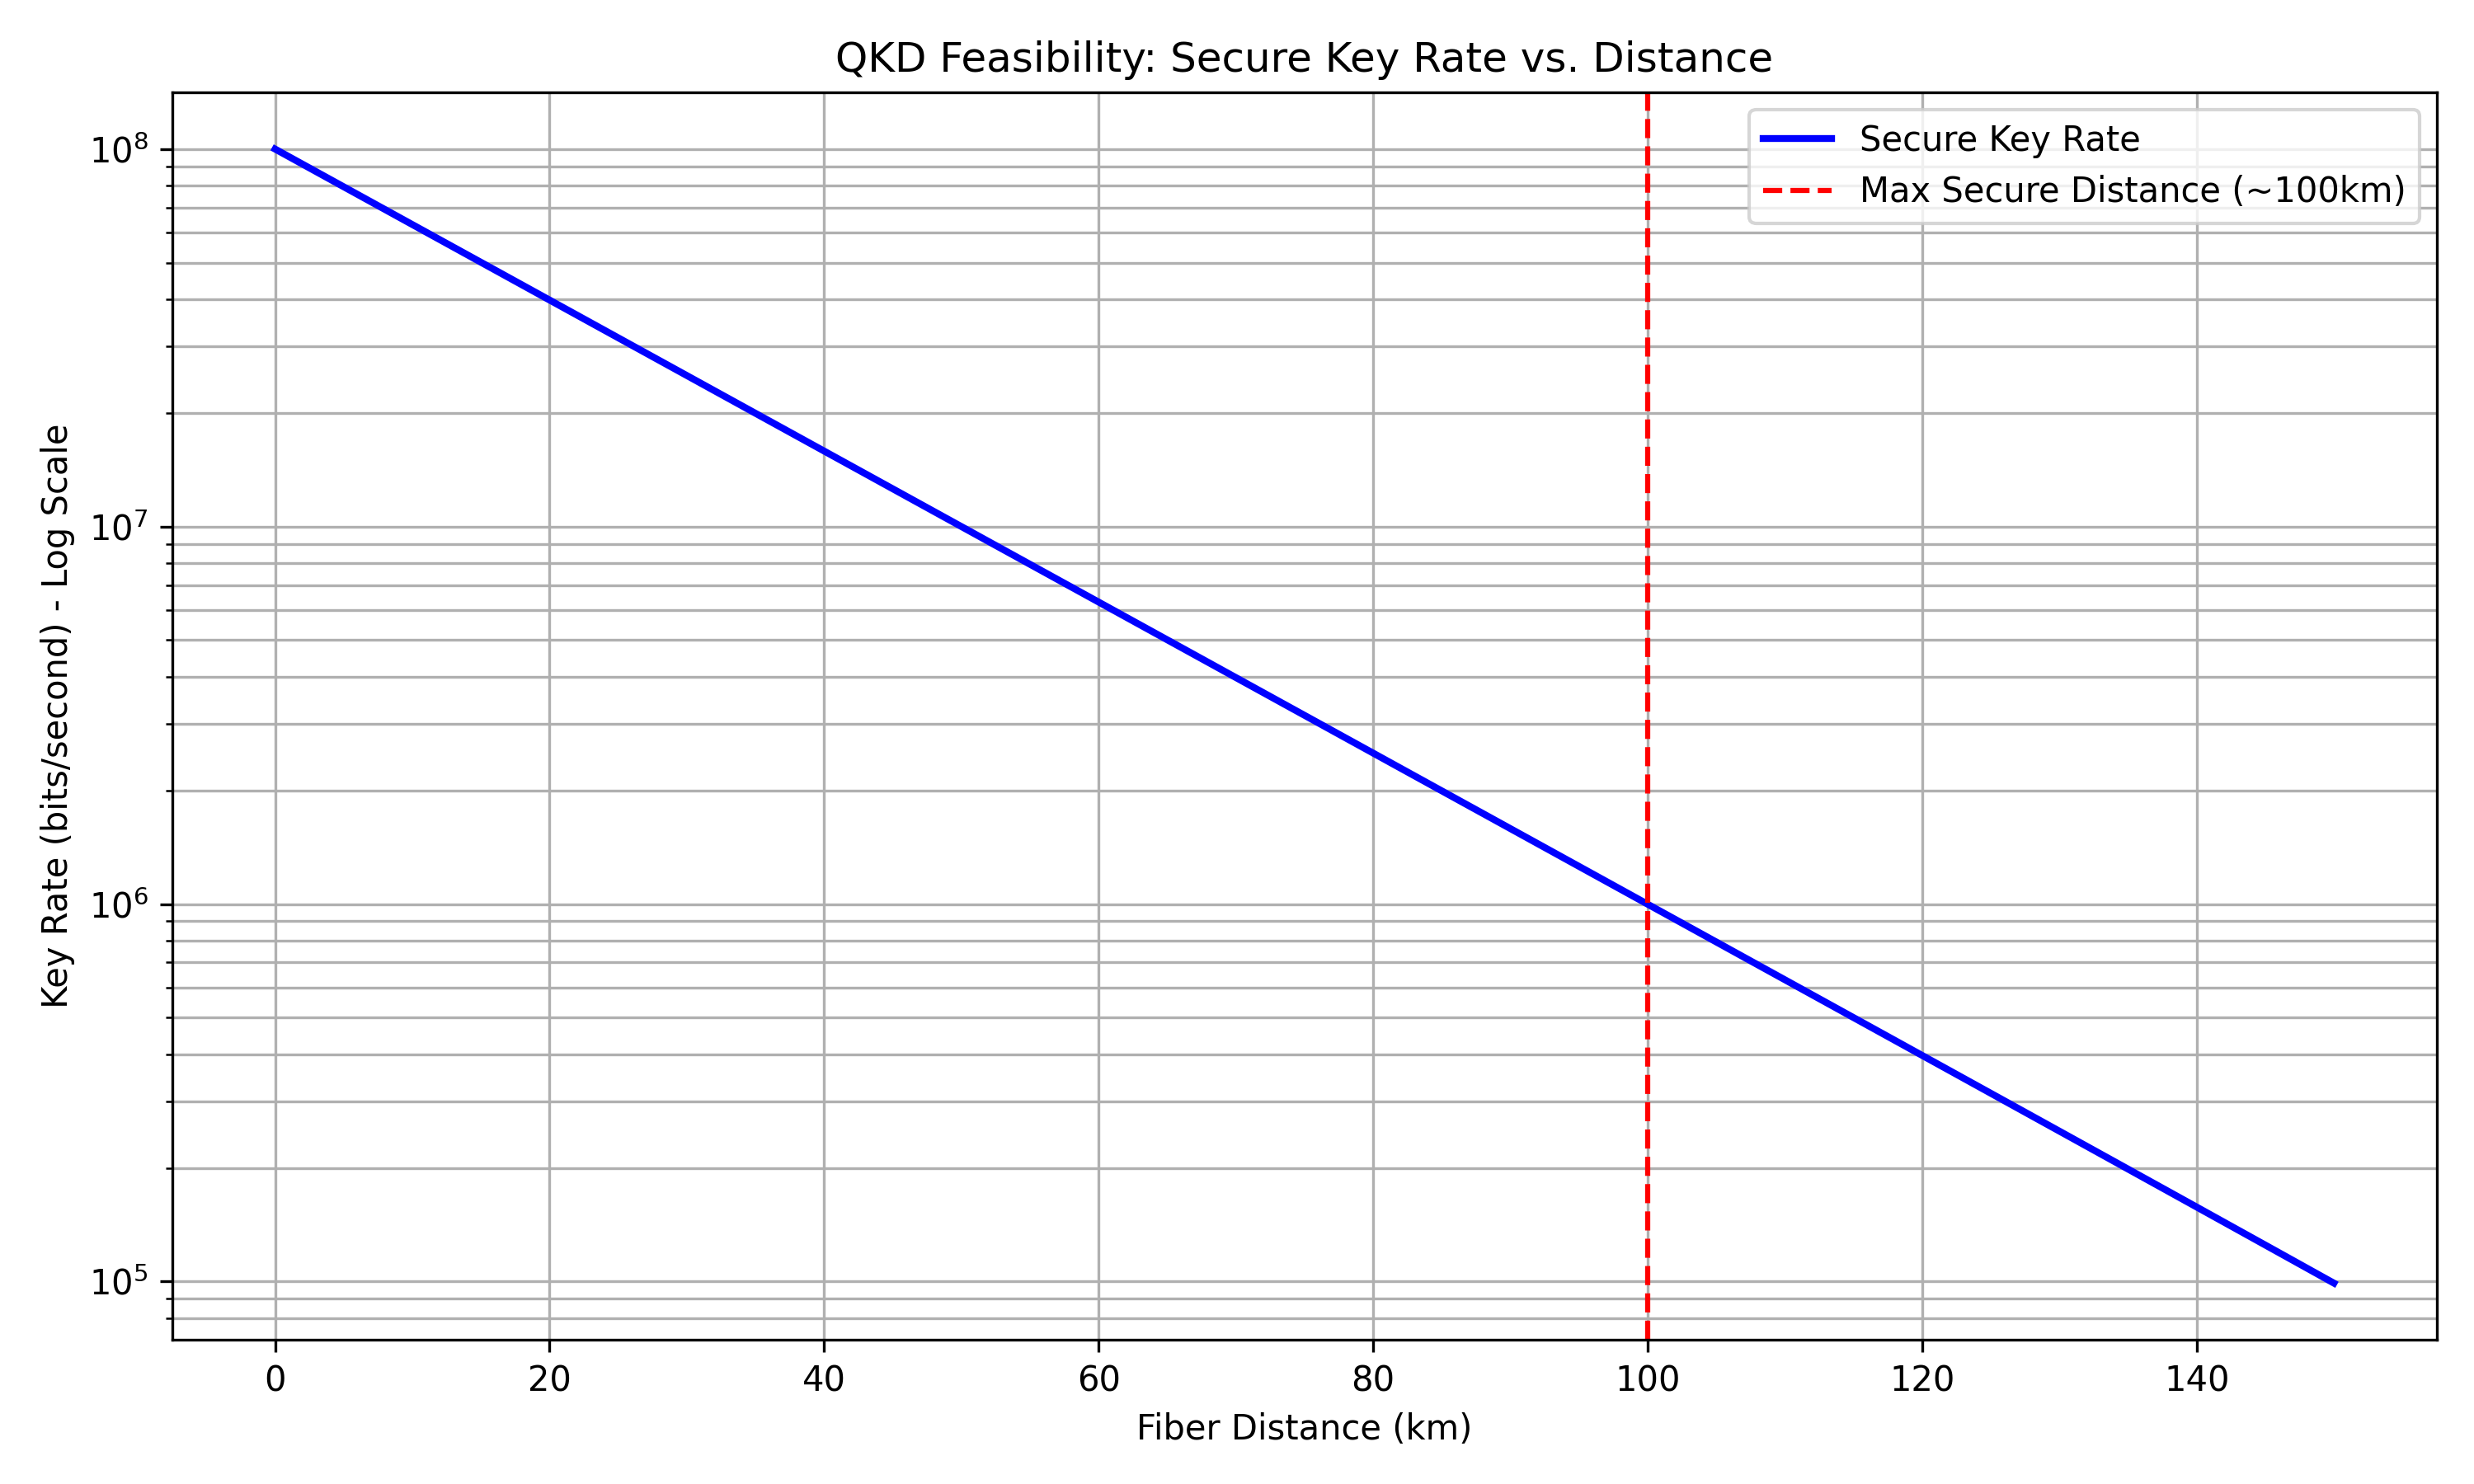
\includegraphics[width=\linewidth]{figures/qkd_skr_vs_distance.png}}
\caption{QKD Secure Key Rate (SKR) versus Fiber Distance (km).}
\label{fig:qkd}
\end{figure}

\subsection{PQC Algorithm Benchmarking}
We benchmarked the performance of Post-Quantum Cryptography algorithms (Kyber and Dilithium) against classical equivalents (RSA and ECC). As shown in Figure \ref{fig:pqc}, Kyber demonstrates highly efficient key encapsulation times while maintaining quantum resistance.

\begin{figure}[htbp]
\centerline{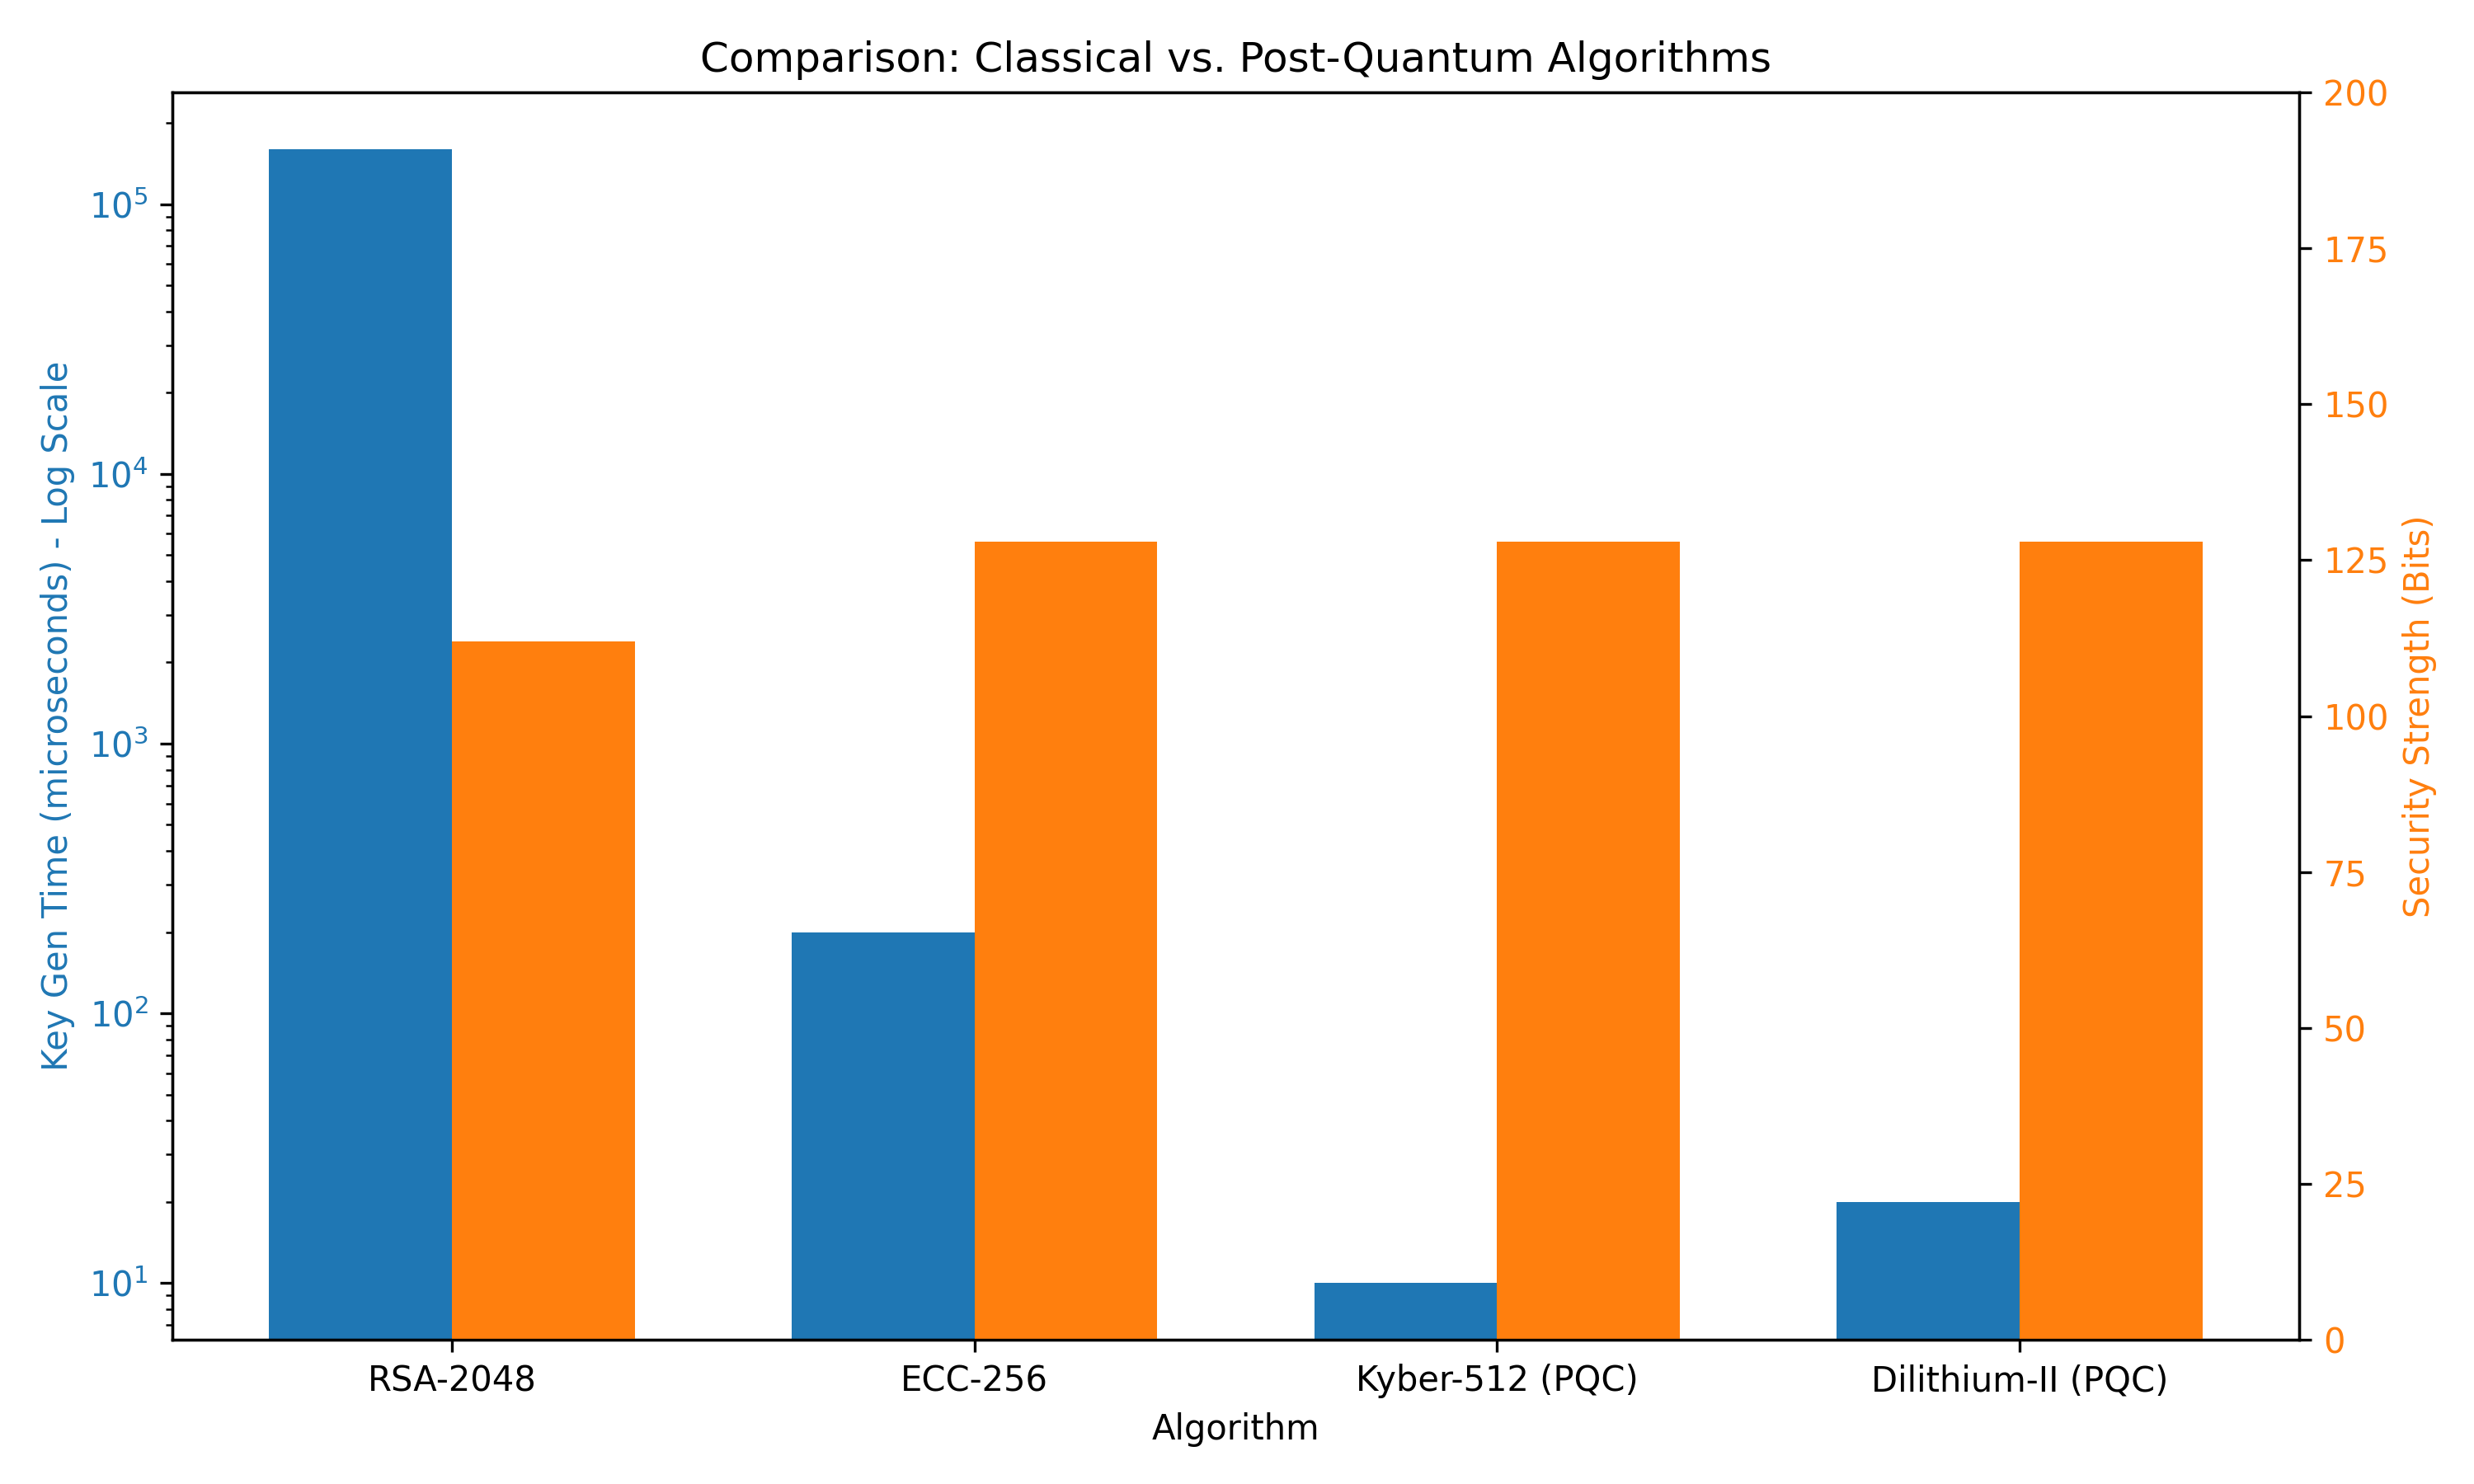
\includegraphics[width=\linewidth]{figures/pqc_comparison.png}}
\caption{Key Generation Time (log scale) of Classical vs. PQC Algorithms.}
\label{fig:pqc}
\end{figure}

\subsection{AI Defense Outcomes}
Both the Random Forest and MLP Neural Network architectures achieved exceptional empirical accuracy ($>$99\%) on the test dataset. Figure \ref{fig:ai_learning} illustrates the learning curve analysis, demonstrating that cross-validation scores converge optimally as the training sample size increases, confirming that neither model is overfitting. Furthermore, the comparative Receiver Operating Characteristic (ROC) curve (Figure \ref{fig:ai_roc_comp}) shows that the Ensemble approach slightly outperforms the Deep Learning approach in maintaining a near-perfect Area Under the Curve (AUC).

\begin{figure}[htbp]
\centerline{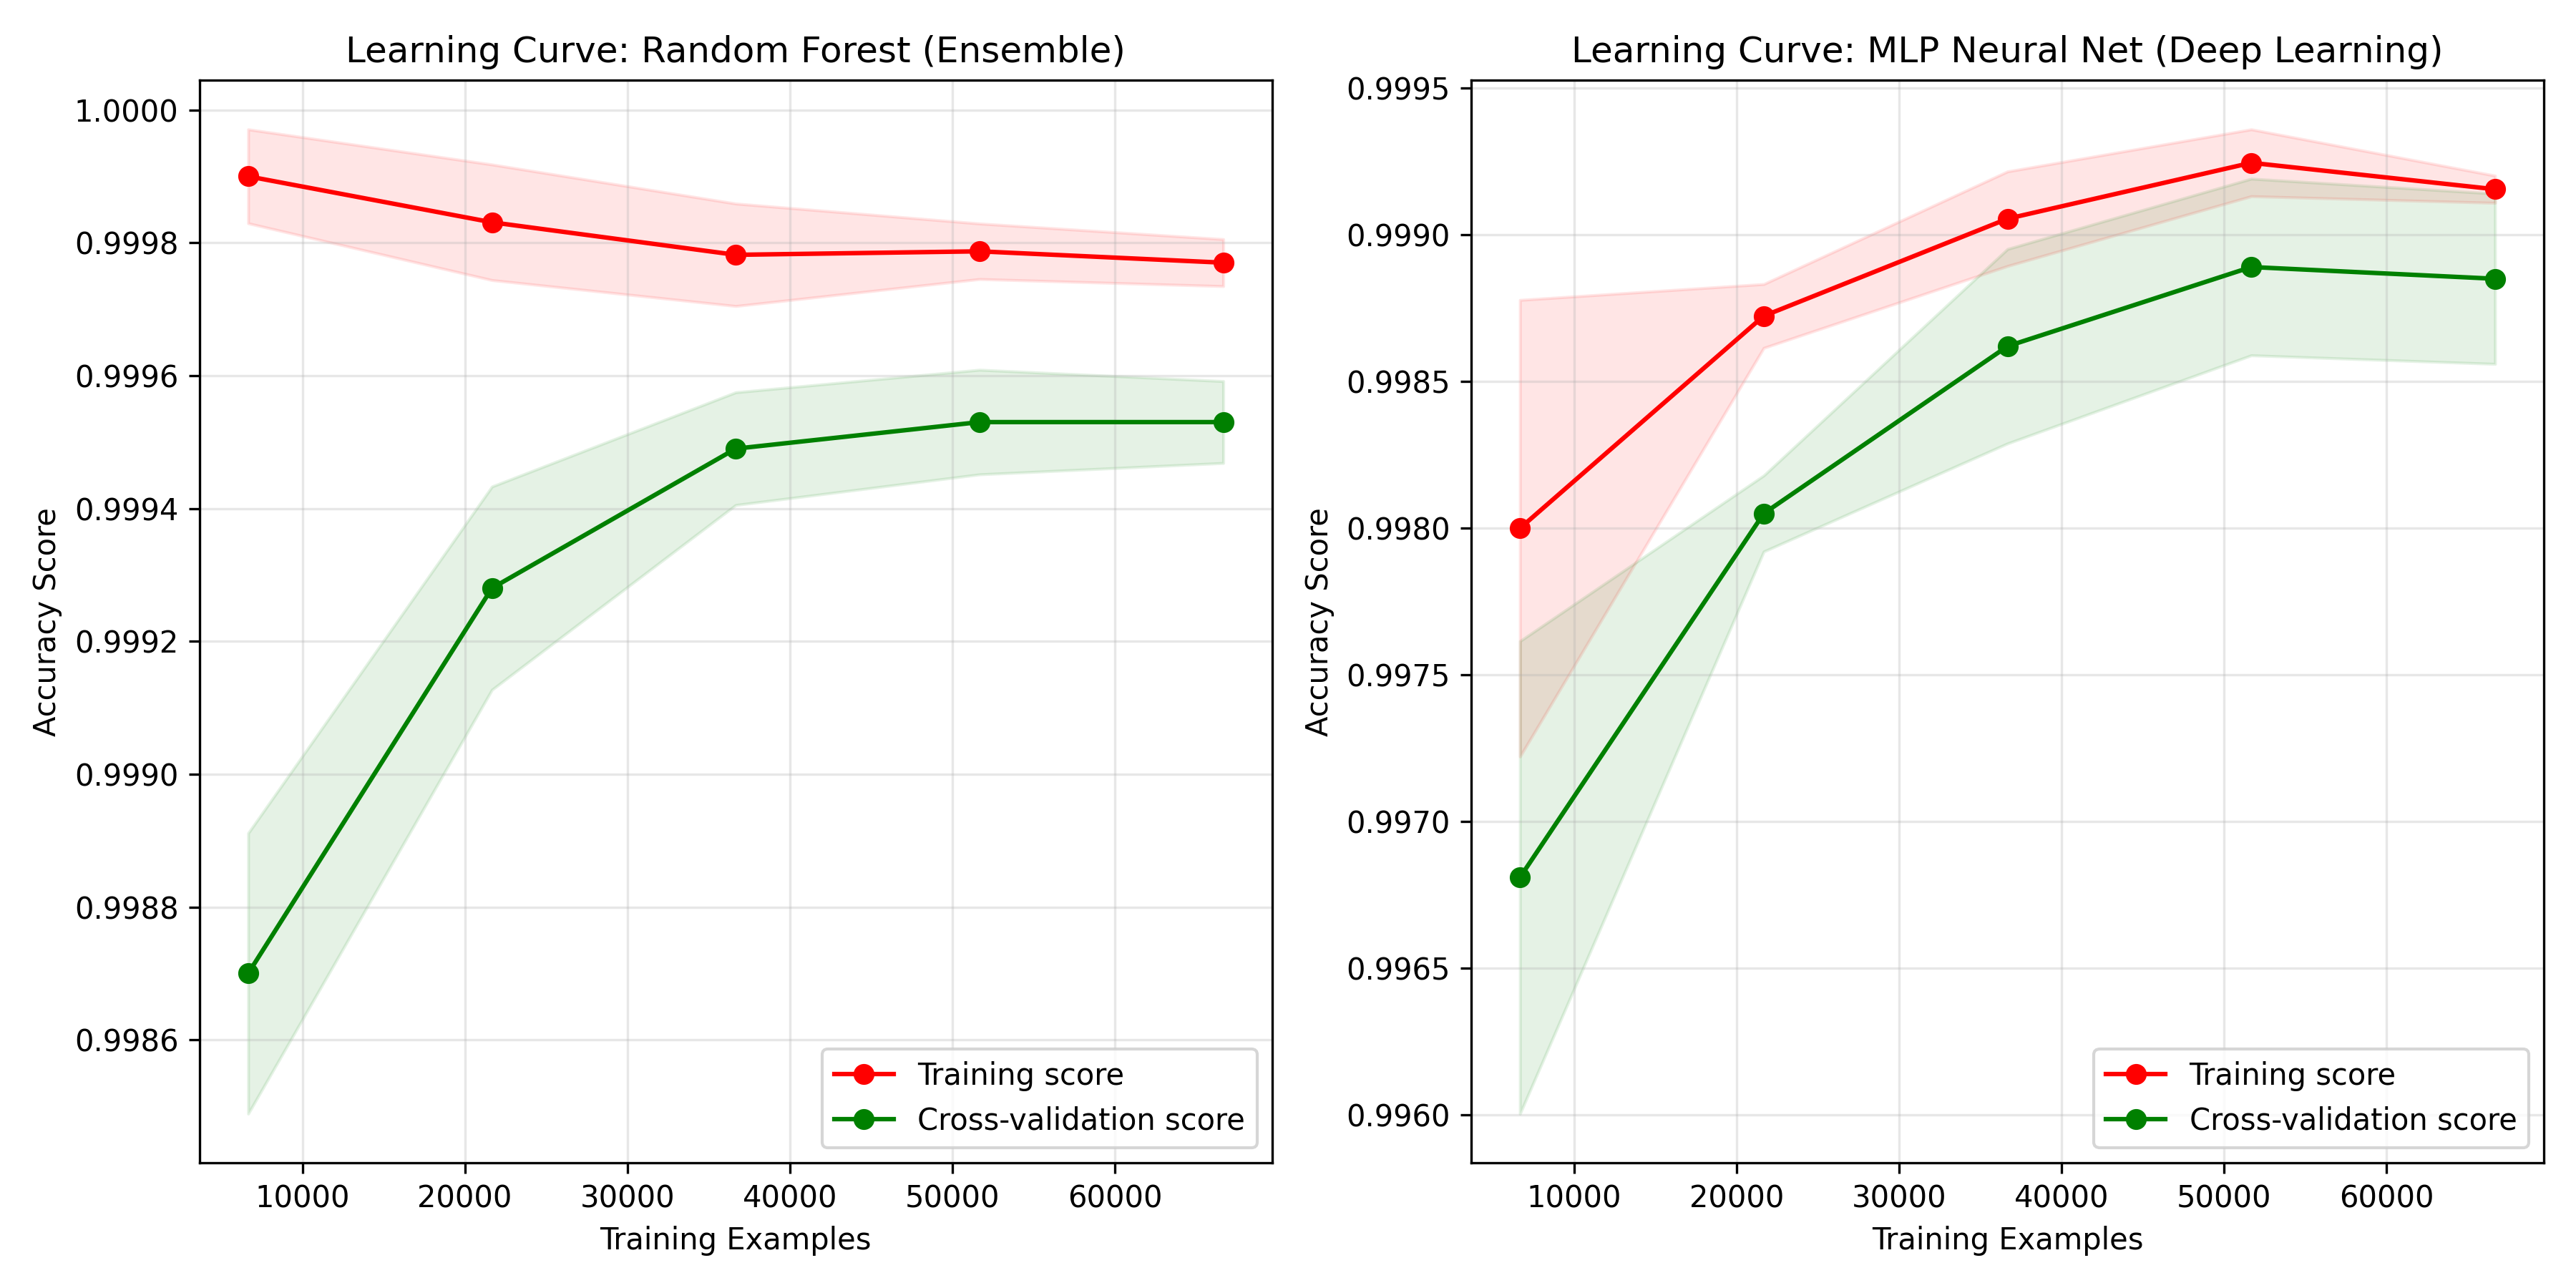
\includegraphics[width=\linewidth]{figures/ai_learning_curve.png}}
\caption{Learning Curve Analysis (Cross-Validation) for both AI architectures.}
\label{fig:ai_learning}
\end{figure}

\begin{figure}[htbp]
\centerline{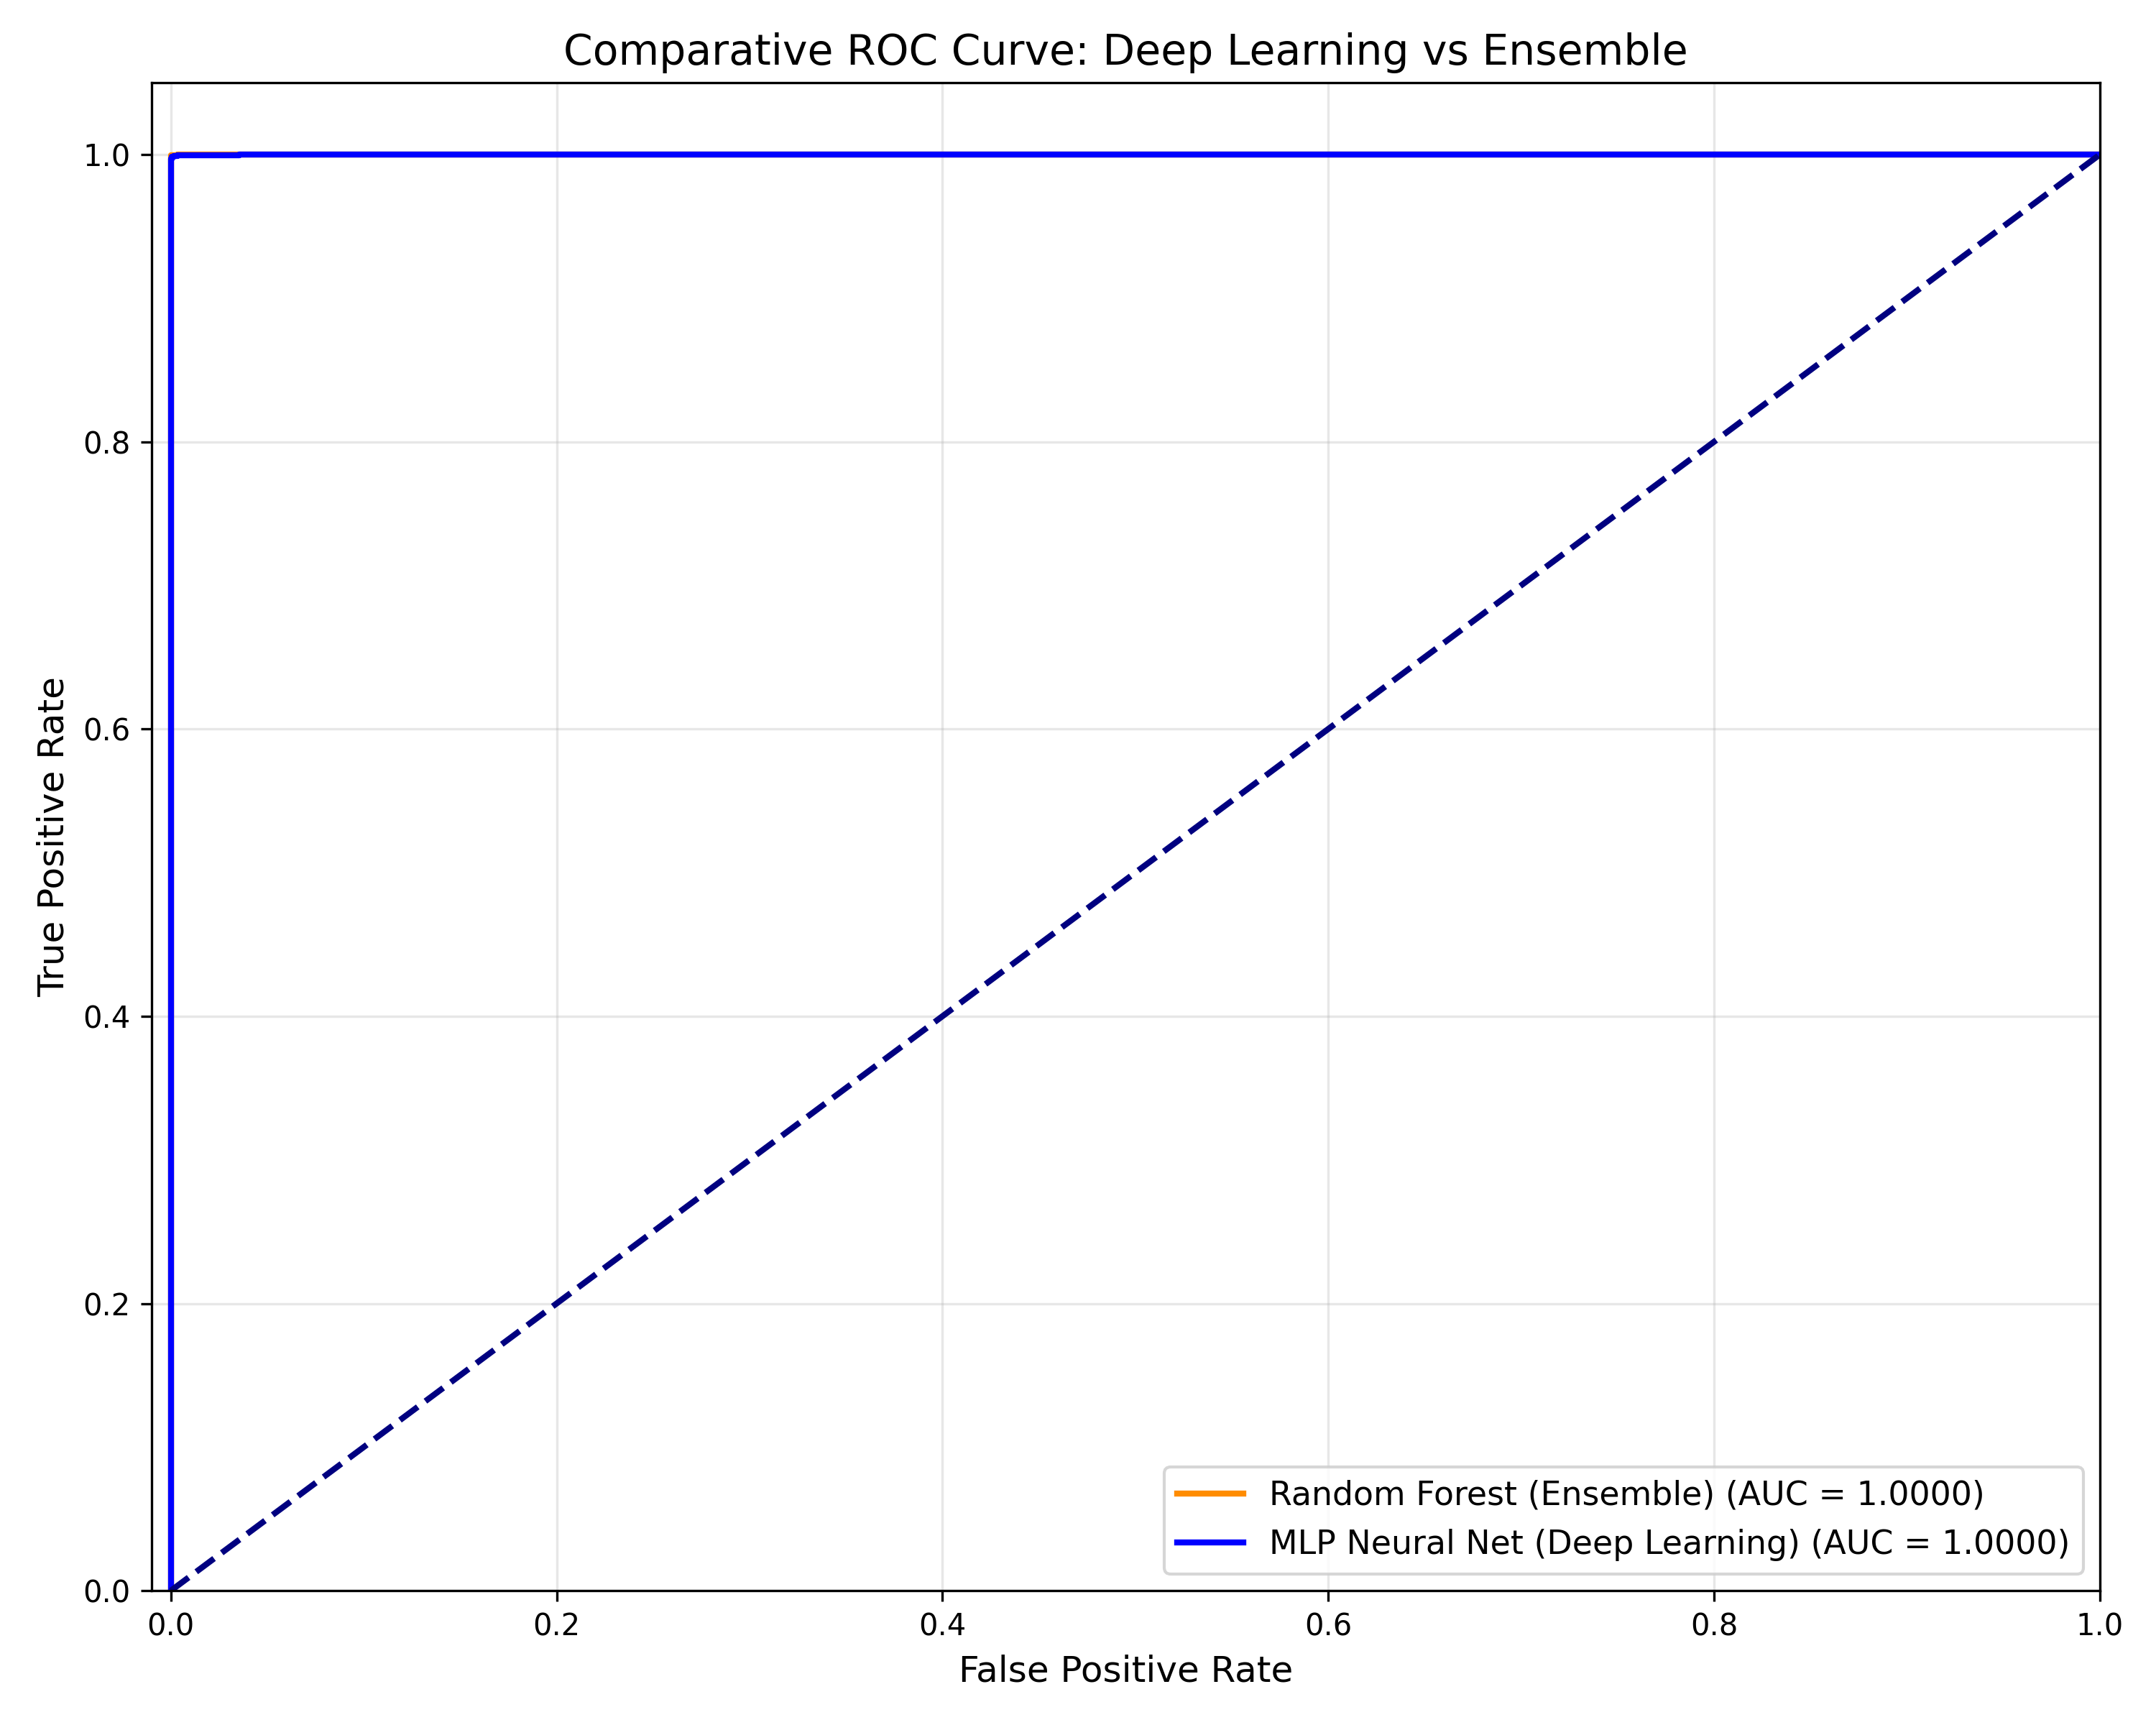
\includegraphics[width=\linewidth]{figures/ai_roc_comparison.png}}
\caption{Comparative ROC Curve: Deep Learning vs Ensemble.}
\label{fig:ai_roc_comp}
\end{figure}

\section{Conclusion}
The proposed architecture provides a robust, quantum-resistant framework for digital health identities. Future work will detail the blockchain integration and the exact consensus mechanisms for off-chain health data.

\bibliographystyle{IEEEtran}
\bibliography{references}

\end{document}
